\documentclass[aspectratio=169,10pt]{beamer}
\usetheme{default}
\usefonttheme{serif}
\usepackage{booktabs,tabularx,array,tikz,pgfplots,xcolor,graphicx}
\usetikzlibrary{arrows.meta,positioning,shapes.geometric}
\pgfplotsset{compat=1.17}

% Palette follows the report: one dark blue, one green for deterministic parts, orange for the model.
\definecolor{bmsblue}{RGB}{0,51,102}
\definecolor{detgreen}{RGB}{34,120,60}
\definecolor{modelorange}{RGB}{200,110,20}
\definecolor{humanred}{RGB}{160,40,40}
\definecolor{pendingorange}{RGB}{180,90,0}
\definecolor{gold}{RGB}{201,151,0}
\definecolor{navy}{RGB}{0,31,77}
\setbeamercolor{structure}{fg=bmsblue}
\setbeamercolor{palette primary}{fg=white,bg=navy}
\setbeamercolor{palette secondary}{fg=white,bg=bmsblue}
\setbeamercolor{palette tertiary}{fg=white,bg=bmsblue!85!black}
\setbeamercolor{palette quaternary}{fg=white,bg=navy}
\setbeamercolor{title}{fg=white,bg=bmsblue}
\setbeamercolor{frametitle}{fg=white,bg=bmsblue}
\setbeamercolor{block title}{fg=white,bg=bmsblue}
\setbeamercolor{block body}{bg=bmsblue!7}
\setbeamercolor{alerted text}{fg=gold!80!black}
\setbeamercolor{item}{fg=gold!85!black}
\setbeamercolor{itemize item}{fg=gold!85!black}
\setbeamercolor{itemize subitem}{fg=bmsblue}
\setbeamercolor{enumerate item}{fg=gold!85!black}
\setbeamercolor{section in head/foot}{fg=white,bg=bmsblue}
% Thin gold rule under the frame title and a navy band above the footline.
\setbeamertemplate{navigation symbols}{}
\setbeamerfont{frametitle}{size=\Large,series=\bfseries}
\setbeamertemplate{frametitle}{%
  \nointerlineskip
  \begin{beamercolorbox}[wd=\paperwidth,ht=1.15cm,dp=0.35cm,leftskip=0.7cm,rightskip=0.7cm]{frametitle}
    \usebeamerfont{frametitle}\insertframetitle\hfill{\normalfont\scriptsize\color{gold}\insertsection}
  \end{beamercolorbox}
  \nointerlineskip
  {\color{gold}\rule{\paperwidth}{2.2pt}}
  \vskip 0.25cm}
\setbeamertemplate{footline}{%
  \leavevmode
  \begin{beamercolorbox}[wd=\paperwidth,ht=0.3cm,dp=0.25cm,leftskip=0.7cm,rightskip=0.7cm]{palette primary}
    \scriptsize ReCycleGuard\hfill B.M.S. College of Engineering\hfill\insertframenumber{} / \inserttotalframenumber
  \end{beamercolorbox}}
\setbeamersize{text margin left=0.9cm,text margin right=0.9cm}

\newcommand{\pending}[1]{{\color{pendingorange}\textbf{[#1: to be completed]}}}
\newcommand{\code}[1]{\texttt{\small #1}}

\title[ReCycleGuard]{ReCycleGuard}
\subtitle{An Agentic Assistant for Auditable E-Waste EPR Compliance Reconciliation}
\author[Team]{%
  1BM23CD020 H Sampreeth Bhat \and 1BM23CD047 R V Abhishek (Team Lead) \and
  1BM23CD063 Sushanth S \and 1BM23CD069 Vedantha Vinay Vernekar}
\institute[BMSCE]{B.M.S. College of Engineering, Bengaluru\\Department of CSE (Data Science)\\
Agentic AI (26CD7PEAAI), Final Review}
\date{November 2026}
\titlegraphic{
\includegraphics[height=1.6cm]{logo.png}}

\begin{document}

{\setbeamercolor{background canvas}{bg=navy}
\begin{frame}[plain]
\begin{tikzpicture}[remember picture,overlay]
\fill[gold] ([yshift=-1.55cm]current page.north west) rectangle ([yshift=-1.63cm]current page.north east);
\fill[gold] ([yshift=1.55cm]current page.south west) rectangle ([yshift=1.63cm]current page.south east);
\node[anchor=north east,xshift=-0.6cm,yshift=-0.2cm] at (current page.north east) {
\includegraphics[height=1.2cm]{logo.png}};
\node[anchor=north west,xshift=0.6cm,yshift=-0.55cm,text=white] at (current page.north west) {\scriptsize B.M.S. College of Engineering \textbullet\ Department of CSE (Data Science)};
\end{tikzpicture}
\vfill
\centering
{\color{white}{\fontsize{34}{38}\selectfont\bfseries ReCycleGuard}\\[6pt]
{\large An Agentic Assistant for Auditable E-Waste EPR Compliance Reconciliation}\\[4pt]
{\color{gold}\rule{6cm}{1pt}}\\[8pt]
{\small Agentic AI (26CD7PEAAI), Final Review, November 2026}\\[10pt]
{\footnotesize 1BM23CD020 H Sampreeth Bhat \quad 1BM23CD047 R V Abhishek (Team Lead)\\
1BM23CD063 Sushanth S \quad 1BM23CD069 Vedantha Vinay Vernekar}}
\vfill\vspace{0.6cm}
\end{frame}}

\section{Problem}
\begin{frame}{Problem and the decision supported}
\begin{itemize}
\item Indian producers of electronics must meet recycling obligations under the E-Waste (Management) Rules, 2022 by buying EPR credits from registered recyclers.
\item The officer must show that, for each metal, the obligation, certificates, transfers, payments and portal balance agree.
\item The records live in PDFs, ledgers and a portal export, and they disagree in specific ways.
\end{itemize}
\begin{block}{Decision supported}
Which discrepancy should the compliance officer investigate next, and what verification or corrective action does the evidence support?
\end{block}
\small The output is an advisory working paper for a human reviewer. It is not a filing, a legal verdict or a fraud finding.
\end{frame}

\begin{frame}{Why a record discrepancy is hard to read}
\begin{columns}[T]
\column{0.5\textwidth}
\textbf{Typical faults}
\begin{itemize}
\item overlapping exports count a transfer twice
\item tonnes mixed into kilograms
\item an unregistered entity alias on an invoice
\item cancelled or expired certificates still counted
\item payment made but the portal transfer never completed
\item a memo read as an official deadline extension
\end{itemize}
\column{0.5\textwidth}
\textbf{Why not a script or one prompt}
\begin{itemize}
\item A script cannot choose what to check next.
\item A single prompt cannot calculate exactly or cite reliably.
\item The useful number of steps varies by case, and a stopping rule is needed.
\end{itemize}
\end{columns}
\end{frame}

\section{Design}
\begin{frame}{Architecture}
\centering
\resizebox{0.97\linewidth}{!}{%
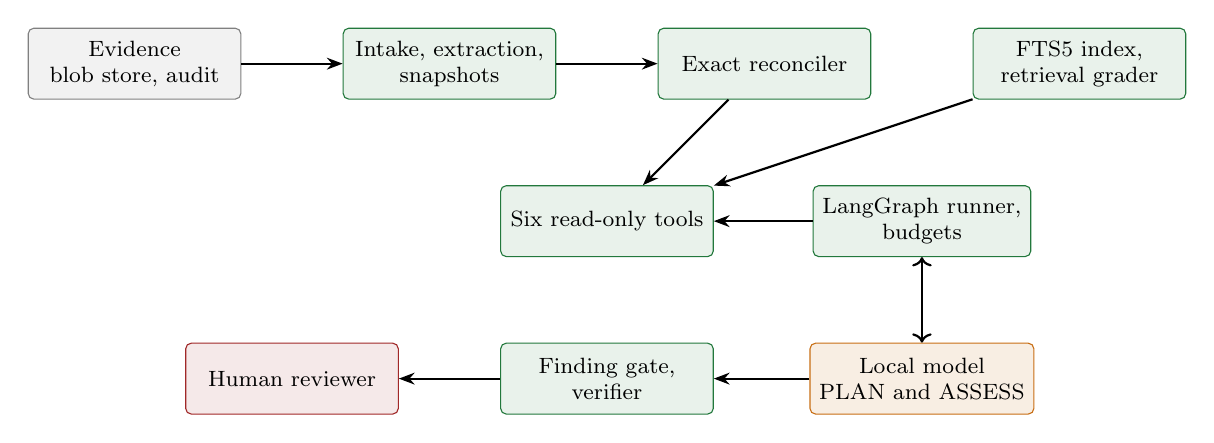
\begin{tikzpicture}[
  det/.style={draw=detgreen,fill=detgreen!10,rounded corners=2pt,minimum width=2.7cm,minimum height=0.9cm,align=center,font=\footnotesize},
  llm/.style={draw=modelorange,fill=modelorange!12,rounded corners=2pt,minimum width=2.7cm,minimum height=0.9cm,align=center,font=\footnotesize},
  hum/.style={draw=humanred,fill=humanred!10,rounded corners=2pt,minimum width=2.7cm,minimum height=0.9cm,align=center,font=\footnotesize},
  st/.style={draw=gray,fill=gray!10,rounded corners=2pt,minimum width=2.7cm,minimum height=0.9cm,align=center,font=\footnotesize},
  arr/.style={-{Stealth[length=2mm]},thick}]
\node[st] (ev) at (0,0) {Evidence\\blob store, audit};
\node[det] (ing) at (4,0) {Intake, extraction,\\snapshots};
\node[det] (rec) at (8,0) {Exact reconciler};
\node[det] (idx) at (12,0) {FTS5 index,\\retrieval grader};
\node[det] (tools) at (6,-2.0) {Six read-only tools};
\node[det] (run) at (10,-2.0) {LangGraph runner,\\budgets};
\node[llm] (mod) at (10,-4.0) {Local model\\PLAN and ASSESS};
\node[det] (gate) at (6,-4.0) {Finding gate,\\verifier};
\node[hum] (rev) at (2,-4.0) {Human reviewer};
\draw[arr] (ev) -- (ing);
\draw[arr] (ing) -- (rec);
\draw[arr] (idx) -- (tools);
\draw[arr] (rec) -- (tools);
\draw[arr] (run) -- (tools);
\draw[arr,<->] (run) -- (mod);
\draw[arr] (mod) -- (gate);
\draw[arr] (gate) -- (rev);
\end{tikzpicture}}

\vspace{2pt}\footnotesize Green: deterministic code. Orange: the model. Red: the human decision. The model proposes, code decides what is accepted.
\end{frame}

\begin{frame}{The agent loop}
\begin{columns}[T]
\column{0.55\textwidth}
\begin{enumerate}
\item \textbf{Preflight} (no model): missing pages stop the run.
\item \textbf{PLAN}: the model proposes one check or a stop.
\item \textbf{Act}: a whitelisted tool runs (exact decimals or retrieval).
\item \textbf{ASSESS}: the model judges the observation: supports, refutes, weak, no progress, unknown.
\item Continue, resolve or abstain. \code{RESOLVE} requires \code{SUPPORTS}.
\item Draft, verify (one repair), then \textbf{human review}.
\end{enumerate}
\column{0.43\textwidth}
\begin{block}{Bounds}
12 model calls, 600 s, token reservation checked before dispatch; 8 tool calls and 2 reformulations per finding; repeat actions stopped by a fingerprint.
\end{block}
\small Each turn is committed with a compare-and-swap version, so a killed run resumes without repeating a tool call.
\end{columns}
\end{frame}

\begin{frame}{Division of labour between the model and the code}
\begin{tabularx}{\linewidth}{@{}p{0.2\linewidth} X X@{}}
\toprule
 & \textbf{Model may} & \textbf{Model may not} \\ \midrule
Quantities & read results of exact tools & compute, state or alter a number \\
Evidence & choose what to inspect next & approve evidence or edit originals \\
Findings & attach one proposal & bypass the gate (citations, digits, wording) \\
Tools & pick from six read-only tools & run code, SQL, shell, or write \\
Decision & assess and abstain & act as reviewer or issue a legal verdict \\
\bottomrule
\end{tabularx}
\end{frame}

\begin{frame}{Six audited tools}
\small
\begin{tabularx}{\linewidth}{@{}l X@{}}
\toprule
\textbf{Tool} & \textbf{Purpose} \\ \midrule
\code{inspect\_evidence} & parsed fields and exact locators of observations \\
\code{lookup\_locator} & verified provision text at a legal path \\
\code{trace\_certificate} & lifecycle: issued, transferred, cancelled, expired \\
\code{compute\_reconciliation} & required, supported, gap, pending per bucket \\
\code{compare\_return} & portal claims against ledger-supported balances \\
\code{search\_rules} & BM25 passages graded for authority and date \\
\bottomrule
\end{tabularx}

\medskip\small Each call stores an intent record before it runs and a result record after it completes.
\end{frame}

\section{Safety}
\begin{frame}{Safety and guardrails}
\begin{itemize}
\item \textbf{Untrusted text:} dossier and retrieved text enter the prompt as escaped JSON; a benchmark family inserts an override instruction into an invoice remark.
\item \textbf{Finding gate:} citations must be evidence this run returned; no digits, prohibited or authority wording.
\item \textbf{No blind retry:} an uncertain model-call outcome ends the run; every attempt is kept.
\item \textbf{Host sandbox:} macOS profile, loopback-only network, probes must all be denied before start (1,630 of 1,630 denied in the final run).
\item \textbf{Human review:} the decision is bound to the exact report and input digests.
\end{itemize}
\end{frame}

\section{Evaluation}
\begin{frame}{Data and evaluation protocol}
\begin{columns}[T]
\column{0.5\textwidth}
\textbf{Synthetic benchmark \code{pilot-0.1}}
\begin{itemize}
\item 48 fictional dossiers, 16 fault families
\item 24 development, 24 held-out (sealed, outside the repository)
\item 8 combinations per split
\item references are agent-validated, not hand-reviewed
\end{itemize}
\column{0.5\textwidth}
\textbf{Variants}
\begin{itemize}
\item V0 deterministic, no model
\item SC scripted control
\item V1 fixed retrieval, real model
\item V2 adaptive, real model
\end{itemize}
Primary metric: supported case success. Human rubric: citation, dates, next action (blind to variant).
\end{columns}
\end{frame}

\begin{frame}{Development reliability, prompt v9}
\small
\textbf{24 development dossiers $\times$ V1 and V2, one repeat}\par\smallskip
\begin{tabularx}{\linewidth}{@{}X c c@{}}
\toprule
\textbf{Criterion (threshold)} & \textbf{V1} & \textbf{V2} \\ \midrule
Runs not failed ($\ge$ 90\%) & 24/24 & 24/24 \\
Schema-valid replies per call ($\ge$ 95\%) & 132/132 & 43/43 \\
Call timeouts ($\le$ 5\%) & 0 & 0 \\
Forbidden actions executed (0) & 0 & 0 \\
Mean wall time (V1 $\le$ 120 s, V2 $\le$ 240 s) & \textcolor{humanred}{134 s} & 62 s \\
Mean model calls per run & 5.5 & 1.8 \\
Correct model finding ($\ge$ 1) & \multicolumn{2}{c}{\textcolor{humanred}{not met}} \\
\bottomrule
\end{tabularx}

\vspace{4pt}\footnotesize Development set only; a check of the setup, not a claim of quality. Crash tests: killed runner and killed server both recovered with no repeated trial.
\end{frame}

\begin{frame}{Quality on development dossiers}
\small
\begin{tabularx}{\linewidth}{@{}X c c@{}}
\toprule
 & \textbf{V1} & \textbf{V2} \\ \midrule
Exact reconciliation (reviewed trials) & 28/28 buckets & 26/26 buckets \\
Primary success (all 24 / reviewed only) & 2 / 1 of 22 & 2 / 1 of 22 \\
Micro precision / recall & 0.67 / 0.21 & 0.67 / 0.15 \\
Model proposals made / accepted / correct & 16 / 1 / 0 & 0 / 0 / 0 \\
\bottomrule
\end{tabularx}

\begin{itemize}
\item Reconciliation is exact because it is deterministic.
\item Fault families found came from deterministic rule and scope checks (F11, F12, F14).
\item 14 of 16 proposals were refused for authority wording; the one accepted finding was a false positive.
\end{itemize}
\end{frame}

\begin{frame}{Prompt development on the tuning set}
\begin{columns}[T]
\column{0.5\textwidth}
\small
\begin{tabularx}{\linewidth}{@{}l X@{}}
\toprule
\textbf{Version} & \textbf{Effect} \\ \midrule
v5, v6 & invented ids: 29, then 40 of 48 not failed \\
v7 & 100\% schema-valid, no proposals \\
v8 & 40 invalid attempts: proposal at the wrong level \\
v9 & 13 V1 proposals, 1 accepted \\
\bottomrule
\end{tabularx}
\column{0.5\textwidth}
\begin{itemize}
\item Tuned only on 16 development cases; 8 checking cases run once afterwards.
\item Each fix moved the failure to the next layer.
\item Success rate did not change (2 of 16).
\end{itemize}
\end{columns}
\end{frame}

\section{Experiment}
\begin{frame}{Experiment: fixed versus adaptive investigation}
\begin{block}{Hypothesis H1}
On the same dossiers, tools, corpus and budget, V2 has a higher supported case-success rate than V1 at comparable cost.
\end{block}
\begin{itemize}
\item 24 held-out dossiers (two are expected preflight stops, reported with and without).
\item Order of V1 and V2 alternates by case; repeats $R$ fixed at the freeze, before any held-out run.
\item Paired case-level bootstrap with all repeats of a case resampled together.
\item Development evidence: V2 uses about one third of the model calls and is not more successful.
\end{itemize}
\end{frame}

\begin{frame}{Held-out result}
\centering
\begin{tabularx}{0.8\linewidth}{@{}l c c c@{}}
\toprule
\textbf{Variant} & \textbf{Success rate} & \textbf{95\% interval} & \textbf{Calls per run} \\ \midrule
V0 & {\color{pendingorange}\textbf{pending}} & {\color{pendingorange}\textbf{pending}} & -- \\
V1 & {\color{pendingorange}\textbf{pending}} & {\color{pendingorange}\textbf{pending}} & {\color{pendingorange}\textbf{pending}} \\
V2 & {\color{pendingorange}\textbf{pending}} & {\color{pendingorange}\textbf{pending}} & {\color{pendingorange}\textbf{pending}} \\
V2 $-$ V1 & \multicolumn{3}{c}{{\color{pendingorange}\textbf{pending}}} \\
\bottomrule
\end{tabularx}

\medskip\small The held-out run waits for a frozen prompt and model setup. No held-out number is shown in this deck.
\end{frame}

\section{Close}
\begin{frame}{Limitations}
\begin{itemize}
\item Synthetic data, a two-source corpus and one small quantised local model.
\item Templates and seeds are in the repository, so the held-out set is not externally blind.
\item One person built, ran and evaluated the system; blind teammate scoring reduces this, and does not remove it.
\item The references were checked by a coding agent, not by a person.
\item The model adds little on the development set; detections come mainly from deterministic checks.
\item Multi-agent collaboration and memory across runs were not built.
\end{itemize}
\end{frame}

\begin{frame}{Conclusion and next steps}
\begin{itemize}
\item A bounded, audited agent loop with exact arithmetic, a gate for model output and mandatory human review.
\item The setup is reliable on development data; quality of the model's findings is the open problem.
\item \textbf{Next:} teach the prompt the substitutes for authority-list wording, tune on a faster runtime, freeze, and run the held-out experiment with the blind rubric.
\item Final conclusion on adaptive investigation: \pending{held-out result}.
\end{itemize}
\end{frame}

\begin{frame}{Team and ownership}
\small
\begin{tabularx}{\linewidth}{@{}l l X@{}}
\toprule
\textbf{USN} & \textbf{Name} & \textbf{Components} \\ \midrule
1BM23CD020 & H Sampreeth Bhat & intake, extraction, index, retrieval, corpus \\
1BM23CD047 & R V Abhishek (Lead) & orchestration, model gateway, sandbox, trial coordinator \\
1BM23CD063 & Sushanth S & reconciler, tools, synthetic generator, dossiers \\
1BM23CD069 & Vedantha Vinay Vernekar & audit kernel, reports, review, export, scoring isolation \\
\bottomrule
\end{tabularx}

\medskip\small Every member is expected to explain the whole system.
\end{frame}

{\setbeamercolor{background canvas}{bg=navy}
\begin{frame}[plain]
\centering\vfill
{\color{white}{\fontsize{30}{34}\selectfont\bfseries Questions}\\[8pt]
{\color{gold}\rule{4cm}{1pt}}\\[8pt]
{\small github.com/R-V-Abhishek/ReCycleGuard, branch \texttt{checkpoint-5}}}
\vfill
\end{frame}}

\end{document}
